% Drawn by scripts/revision3/fig_appendix_taxonomy.py; the .pptx is the
% editable source and is released with the paper.
\begin{figure*}[t]
\centering
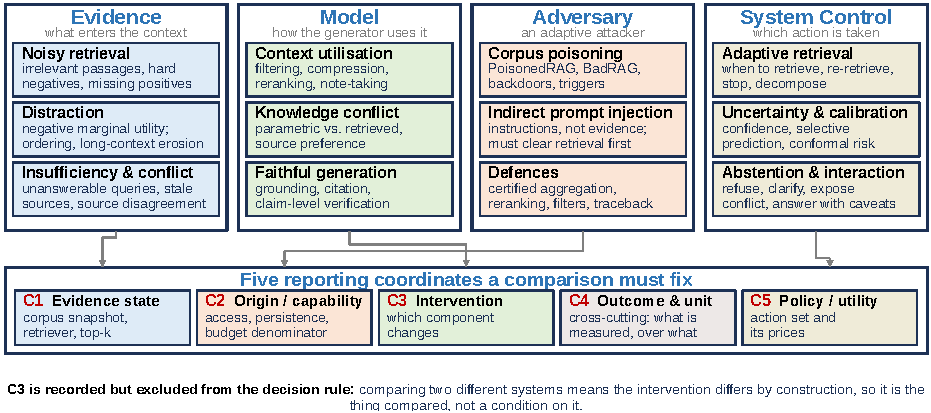
\includegraphics[width=\textwidth]{figures/generated/fig_taxonomy_map.pdf}%
\caption{The four failure surfaces and the reduction they support. Each column
is one surface of the survey (\S\ref{sec:evidence}--\S\ref{sec:system}); the
band below is the five reporting coordinates of \S\ref{sec:coordinates}, and the
connectors show which surface each coordinate collapses. C4 is cross-cutting
and has no single parent surface. The organisation is a partition of the
\emph{comparison} rather than of the literature: the columns tell a reader where
to look for related work, and the band tells a reader what must be stated on
both sides before two numbers can be placed together.}
\label{fig:hierarchical-taxonomy}
\end{figure*}
